\documentclass[brazil,times,12pt]{abnt}
\usepackage[T1]{fontenc}
\usepackage[utf8]{inputenc}
\usepackage{url}
\usepackage{graphicx}
\makeatletter
\usepackage{babel}
\usepackage{url}
\makeatother
\usepackage{listingsutf8}
\usepackage[pdfborder={0 0 0}]{hyperref}

\lstset{
language=Python,
tabsize=2,
inputencoding=utf8,
basicstyle=\scriptsize,
showspaces=false,
showstringspaces=false,
showtabs=false,
% columns=fullflexible
}

\begin{document}

\autor{Pedro Paulo Vezzá Campos}

\titulo{Trabalho Prático 4: Implementação de um Protocolo da Camada de
Transporte}

\comentario{Trabalho apresentado para avaliação na disciplina INE5414, do
curso de Bacharelado em Ciências da Computação, turma 04208, da Universidade   
Federal de Santa Catarina, ministrada pelo professor Carlos Becker Westphall}

\instituicao{Departamento de Informática e Estatística \par Centro
Tecnológico \par Universidade Federal de Santa Catarina}

\local{Santa Catarina - SC, Brasil}

\data{\today}

\capa

\folhaderosto

% \tableofcontents
%\chapter{}
\section*{Resumo}
	Este trabalho apresenta uma implementação do protocolos das camadas de
	rede, transporte e aplicação, com ênfase na segunda. Para demonstrar o
	funcionamento de tais protocolos também foi desenvolvida uma aplicação
	orientada a conexão para apresentar o funcionamento de tais entidades de rede.
	Como forma de fundamentação, também é apresentada uma introdução teórica,
	mostrando os principais conceitos na área dos protocolos e camadas da pilha de
	protocolos do Modelo OSI utilizados durante o trabalho.	

\section*{Introdução}	
	Este quarto trabalho prático possui como objetivo sedimentar os conhecimentos
	apreendidos durante o curso da disciplina, apresentando o desenvolvimento de um
	protocolo de camada de transporte, baseado no exemplo fornecido pela
	bibliografia da disciplina \cite{tanenbaum:redes-computadores}. Como forma de
	mostrar seu funcionamento foram desenvolvidos adicionalmente um protocolo
	orientado a conexão, além das camadas de aplicação e de rede para prover a
	infraestrutura necessária para o funcionamento correto do aplicativo
	desenvolvido.
	
	Este relatório possui a seguinte organização: Primeiramente serão apresentados
	os conceitos principais das camadas de rede, transporte e aplicação da pilha de
	protocolos de redes OSI utilizados durante a implementação da aplicação
	apresentada anteriormente. Posteriormente há uma explanação detalhada dos
	procedimentos adotados para o desenvolvimento da aplicação. Ainda, são
	apresentados alguns comentários e conclusões sobre este trabalho. Por fim é
	apresentado o código fonte comentado da aplicação desenvolvida. 
	
\section*{Camada de Rede}
	No modelo OSI, a camada de rede é a terceira, já no modelo TCP/IP é a segunda.
	Sua tarefa principal é prover serviços à camada de transporte. Para isso, ela
	faz uso das primitivas fornecidas pela camada de enlace de dados.
	
	A camada de rede e a sua camada inferior, a camada de enlace de dados, possuem
	propósitos diferentes. A camada de enlade de dados, tem a
	responsabilidade de transmitir dados entre duas pontas de um canal físico,
	tendo como preocupações questões como a correção de erros, detecção de
	colisões e perdas de datagramas. Já a camada de rede é a responsável
	pela entrega de pacotes da origem ao destino, havendo a possibilidade de ser
	necessário o roteamento entre hosts intermediários. É na camada de rede que
	estão imbutidos os protocolos e algoritmos de roteamento, detecção de
	congestionamento, dentre outros. Ainda, ela é responsável por propiciar uma
	compatibilidade entre redes diferentes, cada uma com configurações variadas.
	Ela possui participação no controle da qualidade de serviço (QoS), além de
	executar funções de controle de erros.

	A camada de rede necessita conhecer diversos parâmetros de configuração para
	poder fornecer um serviço adequado à camada de transporte. Algumas dessas
	informações estão descritas abaixo:
	
	\begin{itemize}
		\item O protocolo de rede é orientado a conexão?
		\item Como controlar o congestionamento da rede?
		\item Quais são os endereços únicos (globais) da rede?
		\item Quais são minhas máquinas vizinhas?
		\item Como devo rotear dados com destino outros computadores?
	\end{itemize}

	Há duas famílias principais de protocolos de rede, os orientados a conexão,
	funcionando por circuitos virtuais e os baseados em datagramas. Cada uma dessas
	abordagens possui vantagens e desvantagens, como é possível ver a seguir:
	
	Protocolos de rede orientados a conexão são mais simples de implementar devido
	a características da própria abordagem, não há a necessidade de controlar
	congestionamento ou utilizar algoritmos sofisticados para oferecer qualidade de
	serviço. Ainda, em tais redes não é necessário que os endereços de origem e
	destino sejam transmitidos em cada pacote. Outra vantagem de se usar
	protocolos de rede baseados em circuitos virtuais é que a possibilidade de
	garantir parâmetros de atraso máximo, garantia essa muito importante para a
	transmissão de dados multimídia, por exemplo. \cite{wiki:network-layer}
	
	Como desvantagem, há um custo ao usar essa escolha: A partir do momento que é
	estabelecido um circuito virtual há a separação de uma porção dos recursos de
	rede exclusivamente para um único usuário, esteja ele usando a rede ou não.
	Isso incorre em custos extra aos provedores de serviços de Internet, sendo
	repassados aos clientes finais, de maneira similar como o que ocorre na
	telefonia convencional.
	
	Já uma camada de rede não orientada a conexão funciona por multiplexação de
	pacotes, ou seja, os pacotes não possuem uma rota pré-estabelecida como ocorre
	no caso anterior após o estabelecimento do circuito virtual. Dessa forma, cada
	pacote deve conter o endereço completo de origem e destino para poder ser
	roteado. Em uma transmissão entre dois computadores os pacotes podem adotar
	diversas rotas diferentes, passando por vários países, por exemplo, dependendo
	da carga da rede no momento do envio do pacote.
	
	Uma grande vantagem de seusar uma camada de rede baseada em datagramas é a sua
	capacidade de distribuir melhor a carga no canal físico, colaborando com menor
	congestionamento em momentos de grande utilização. Além disso, uma rede
	baseada em comutação de pacotes é mais tolerante a falhas uma vez que quando
	um nodo da rede falha os dados podem adotar uma rota alternativa. Um exemplo
	de protocolo de redes não orientado a conexão é o IP
	\cite{wiki:internet-layer}, utilizado na Internet.

\section*{Camada de Transporte}
	A camada de transporte é a terceira camada do modelo TCP/IP e a quarta camada
	segundo o modelo OSI. Ela utiliza os serviços da camada de rede (roteamento de
	pacotes entre hosts, por exemplo) para atender as requisições dos protocolos de
	aplicação.
	
	A camada de transporte tem um papel muito importante dentre as camadas da
	pilha de protocolos OSI. Ela é a primeira camada que estabelece uma conexão
	fim-a-fim, confiável ou não, entre dois processos de aplicação em dois hosts.
	Para um a camada de aplicação (ou sessão, dependendo do modelo), que usa a
	interface da camada de transporte, a conexão de rede pode ser vista como uma
	conexão direta, em que bytes são inseridos em um lado da conexão e após algum
	tempo aparecem no outro lado. O protocolo de transporte é responsável por
	iniciar e terminar as conexões entre processos que desejam estabelecer
	comunicação, fazendo a multiplexação dessas conexões.
	
	É nessa camada que os dados que chegam da camada de sessão são quebrados em
	unidades menores, os pacotes, para que possam ser mais facilmente enviados pela
	camada de rede. Faz parte da responsabilidade de uma camada de transporte que
	forneça uma conexão confiável, por exemplo, garantir que os pacotes cheguem
	ao destino corretamente e em ordem.
	
	O código binário do protocolo de transporte geralmente é o último que
	encontra-se no núcleo (\emph{kernel}) do sistema operacional. As camadas de
	sessão, apresentação e aplicação, quando existentes, geralmente encontram-se em
	espaço de usuário, implementadas como bibliotecas, por exemplo. Programas que
	queriam fazer uso de comunicações HTTP, por exemplo, como um \emph{browser
	web}, utilizam as bibliotecas HTTP para transmitir e receber os dados que por
	ventura devam trafegar pela rede.
	
	Como forma de suportar várias conexões de transporte ao mesmo tempo, o
	software responsável por essa camada de rede possui diversas
	possibilidades:
	
	\begin{description}
  		\item[Multiplexação no tempo] Caso haja apenas uma conexão de rede
  		disponível, a camada de transporte envia dados de diferentes conexões em
  		diferentes períodos de tempo.
  		\item[Exclusividade de conexão] Caso haja alguma aplicação que demande
  		maiores recursos de redes, há a possibilidade que ela monopolize a conexão,
  		de forma a fornecer a melhor qualidade de serviço possível a essa aplicação
  		específica.
  		\item[Escalonamento] Caso haja mais de uma conexão de rede disponível, é
  		possível ainda escalonar a utilização, utilizando algoritmos como o
  		round-robin com as conexões de rede disponíveis, diminuindo assim o
  		congestionamento nas sub-redes que o host está conectado.
	\end{description}
	
\section*{Camada de Aplicação}
	A camada de aplicação é sétima camada no modelo OSI e a quarta no modelo
	TCP/IP. Em ambas é a camada de mais alto nível. Sua característica principal é
	que ela apresenta uma interface direta com os aplicativos. Seu serviço
	é prover a eles uma abstração da comunicação em rede, escondendo os detalhes
	de implementação das camadas mais inferiores. Para isso, ela faz uso da
	camada de apresentação ou de transporte dependendo do modelo de redes
	adotado.

	Exemplos de protocolos da camada de aplicação:
	
	\begin{itemize}
		\item BitTorrent
		\item SSH - \emph{Secure Shell}
		\item BGP - \emph{Border Gateway Protocol}
		\item DHCP - \emph{Dynamic Host Configuration Protocol}
		\item HTTP - \emph{HyperText Transfer Protocol}
		\item DNS - \emph{Domain Name System}
		\item NFS - \emph{Network File System}
		\item FTP - \emph{File Transfer Protocol}
		\item SNMP - \emph{Simple Network Management Protocol}
		\item IMAP - \emph{Internet Message Acces Protocol}
		
	\end{itemize}
	
	A camada de aplicação é responsável transformar os pacotes recebidos da camada
	inferior em informação reconhecível pela aplicação. Os dados passam a ter um
	significado maior que apenas um fluxo de bits. Os programas aplicativos, dentre
	os quais podemos exemplificar os navegadores, players multimídia, clientes de
	IM, dentre outros geralmente usam de bibliotecas para apresentar ao usuário sua
	funcionalidade.
	
	A interface entre os programas de aplicação e os protocolos da camada de
	transporte é feita usando-se \emph{sockets}. Um socket pode ser visto como um
	``tubo'' com um fluxo bidirecional de dados, podendo ter características como
	criptografia, garantia de entrega de informações, etc. As operações disponíveis
	em um \emph{socket} são similares às possíveis de realizar em arquivos.
	Exemplos de operações são o \emph{BIND}, \emph{LISTEN}, \emph{CONNECT},
	\emph{READ} e \emph{WRITE}. Essas operações são a base do funcionamento de um
	socket.


\section*{Desenvolvimento dos protocolos}
	Como informa a bibliografia, que forneceu o código base para a implementação do
	protocolo de transporte:
	
	\begin{quote}
	``Você deve ter em mente a simplicidade da Figura 6.20. Uma entidade de transporte real
	normalmente verificaria a validade de todos os parâmetros fornecidos, cuidaria
	da recuperação do funcionamento após uma falha na camada de rede, trataria das
	colisões de chamadas e seria compatível com um serviço de transporte mais
	genérico, com interrupções, datagramas e versões sem bloqueio das primitivas
	SEND e RECEIVE.'' \cite{tanenbaum:redes-computadores}
	\end{quote}
	
	Dessa forma, a camada de transporte desenvolvida nesse trabalho tem
	características incomuns a uma camada de transporte usual, não implementando o
	TCP nem o UDP, por exemplo. Dessa forma, não é possível usar aplicativos
	normais, tais como \emph{browsers}, ou clientes de e-mail para testar o
	funcionamento da camada de transporte desenvolvida.
	
	Sendo assim, foi desenvolvida uma aplicação orientada a conexão como prova de
	conceito. Tal programa consiste em um programa de bate-papo simples com dois
	clientes distintos em uma mesma janela para melhor visualização. Toda mensagem
	enviada por um cliente é enviada ao outro utilizando a infraestrutura de
	camadas desenvolvida. Como forma de apresentar o funcionamento interno dos
	protocolos, cada cliente pode ver as primitivas invocadas por cada uma das
	camadas desde o envio da mensagem por um lado até a chegada dela no outro lado.
	
\subsection*{Recursos utilizados}
	\begin{description}
	  \item[Ubuntu Linux] Versão 10.10
	  \item[Python 2.7] Linguagem de programação adotada
	  \item[PyQt] Biblioteca utilizada no desenvolvimento da interface gráfica com
	  o usuário.
	\end{description}

\subsection*{Camada de Rede}
	Esta camada possui uma implementação simples neste trabalho. Sua tarefa é de
	realizar o redirecionamento de pacotes enviado por uma camada de transporte
	para a outra. Para isso, a camada de rede fornece a primitiva
	\texttt{enviarPacote} às camadas de transporte. Por outro lado, sempre que um
	novo pacote chega, após a decisão de qual camada de transporte corresponde o
	pacote, é invocado o método \texttt{daRede} correspondente, enviando o dado à
	camada superior.

\subsection*{Camada de Transporte}
	Como descrito anteriormente, a linguagem de programação adotada foi o Python.
	Como o código fornecido pela bibliografia estava programado em C, o primeiro
	passo foi realizar uma tradução para a linguagem destino, realizando diversas
	adaptações necessárias diante da diferença de paradigmas adotados: Estruturado
	vs. Orientado a Objetos, variáveis globais, definições em tempo de compilação,
	etc.
	
	Ainda, o código fornecido teve algumas implementações faltantes suplantadas:
	
	\begin{itemize}
  		\item \texttt{sleep}, e \texttt{wakeUp} que no programa final tornaram-se
  		\texttt{dormir} e \texttt{acordar}, cumprem a função de uma barreira da
  		programação concorrente, bloqueando e reiniciando o funcionamento da camada
  		de transporte à medida que haja novos eventos para serem tratados.
  		\item \texttt{fromNet}, e \texttt{toNet} que no programa final tornaram-se
  		\texttt{daRede} e \texttt{paraRede}, que são métodos de interface com a
  		camada de rede para o recebimento e envio de pacotes.
	\end{itemize}
	
	Para permitir a interação entre camadas vizinhas houve a necessidade que cada
	camada tivesse referências às suas vizinhas para permitir um funcionamento
	síncrono.
	
	A camada de transporte possui um vetor que armazena e organiza as conexões
	atuais, representadas como objetos do tipo \texttt{Conexao}. Cada pacote é
	representado por objeto da classe \texttt{Pacote}, além disso e eles são
	enviados à camada de rede através do método interno \texttt{paraRede}, são
	roteados pela camada de rede, e depois ressurgem na camada de transporte
	homóloga através do método \texttt{daRede}.


\subsection*{Camada de Aplicação}
	A camada de apresentação provê as primitivas básicas ao programa de bate-papo a
	ser apresentado posteriormente. Seus métodos principais são \texttt{conectar}, \texttt{escutar},
	\texttt{enviarMensagem}, \texttt{receberMensagem} e \texttt{fecharConexao}.
	Tais métodos são responsáveis por estabelecer uma conexão, permanecer
	aguardando uma nova conexão, enviar uma mensagem, receber uma mensagem que será
	posteriormente entregue à aplicação e encerrar uma conexão estabelecida,
	respectivamente. Todos esses serviços prestados pela camada de aplicação
	utilizam primitivas fornecidas pela camada de transporte.
	
	
\subsection*{Aplicação Prova de Conceito}
	Como explicado anteriormente, foi desenvolvida um programa de bate-papo
	simples com dois clientes distintos em uma mesma janela para melhor
	visualização. Toda mensagem enviada por um cliente é enviada ao outro
	utilizando a infraestrutura de camadas desenvolvida.
	
	Adicionalmente, como forma de apresentar o funcionamento interno dos
	protocolos, cada cliente pode ver as primitivas invocadas por cada uma das
	camadas desde o envio da mensagem por um lado até a chegada dela no outro
	lado.
	
	%\usepackage{graphics} is needed for \includegraphics
	\begin{figure}[htp]
	\begin{center}
	  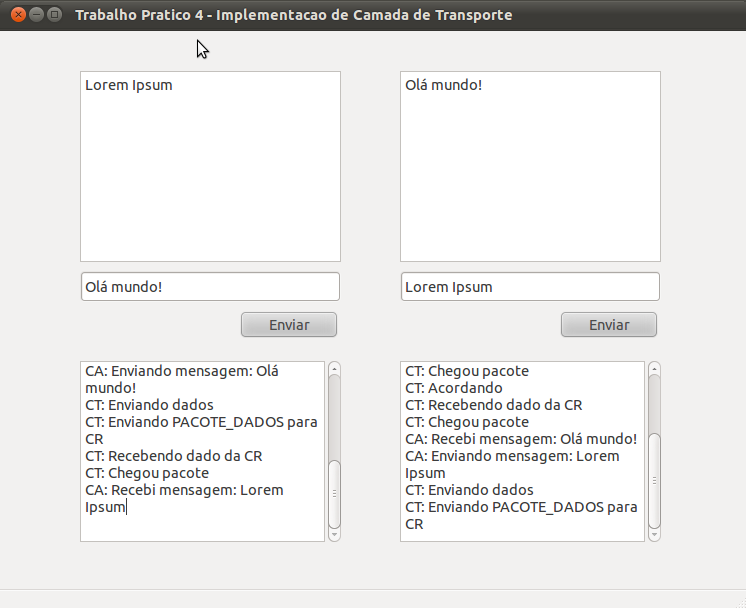
\includegraphics[width=100mm]{imagens/Aplicativo.png}
	  \caption[aplicativo]{Imagem do funcionamento do aplicativo de prova de
	  conceito}
	  \label{aplicativo}
	\end{center}
	\end{figure}


\subsection*{Validação, Verificação e Testes}
	A validação e a verificação foram feitas através de máquinas de estados
	representando o protocolo implementado. Posteriormente à implementação,
	procedeu-se com a codificação de testes unitários através daa biblioteca
	PyUnit, embutida na linguagem Python. Através destes testes unitários
	verificou-se o funcionamento adequado dos protocolos programados.

\section*{Comentários sobre os resultados obtidos}
	O quarto trabalho prático de INE5414 foi de grande importância para a
	sedimentação dos conceitos vistos durante o semestre, contribuindo para o
	objetivo de relacionar teoria e prática em Redes de Computadores. Ainda,
	permitiu elucidar vários conceitos, principalmente os relacionados ao modelo de
	redes em camada, o desenvolvimento de protocolos e suas relações com a
	Engenharia de Software.
	
	Apesar dos protocolos e programa produzidos para esse trabalho possuirem apenas
	caráter didático e não de uso estritamente prático, ainda assim, são
	importantes ferramentas no aprendizado prático dos conceitos vistos em aula.

\section*{Conclusões}
	Neste trabalho, após uma breve introdução ao problema proposto, foi apresentado
	inicialmente uma fundamentação teórica em três importantes camadas do modelo
	OSI e do modelo TCP/IP. 
		
	Posteriormente foram apresentadas as principais características do
	desenvolvimento de um protocolo de transporte orientado a conexão, além de
	suas camadas vizinhas e de uma aplicação de bate-papo, como prova de conceito.
	Além disso foram explicados os passos de verificação, validação e testes
	empregados durante o desenvolvimento do programa.
	
	Por fim, foram apresentados comentários a respeito do trabalho e o código fonte
	comentado resultante. 
	
\section*{Código fonte}
	\subsection*{Inicialização do programa}
	\lstinputlisting{src/main.py}
	
	\subsection*{Camada de Aplicação}
	\lstinputlisting{src/camadaAplicacao.py}
	
	\subsection*{Camada de Transporte}
	\lstinputlisting{src/camadaTransporte.py}
	
	\subsection*{Pacote}
	\lstinputlisting{src/pacote.py}
	
	\subsection*{Camada de Rede}
	\lstinputlisting{src/camadaRede.py}

	\subsection*{Testes}
	\lstinputlisting{src/testes.py}
	
	\subsection*{Interface Gráfica}
	\lstinputlisting{src/interface/interface.py}
	\lstinputlisting{src/interface/layoutInterface.py}

\bibliographystyle{abnt-num}
\bibliography{bibliografia}
\end{document}